\documentclass[12pt,a4paper]{report}

\usepackage[utf8]{inputenc}
\usepackage[T1]{fontenc}
\usepackage[french]{babel}
\usepackage{geometry}
\usepackage{xcolor}
\usepackage{graphicx}
\usepackage{hyperref}
\usepackage{enumitem}
\usepackage{array}
\usepackage{longtable}
\usepackage{float}
\usepackage{listings}

\geometry{margin=2.5cm}
\hypersetup{
    colorlinks=true,
    linkcolor=blue!60!black,
    urlcolor=blue!60!black
}

\definecolor{primary}{HTML}{1E3A8A}
\definecolor{lightgray}{HTML}{F3F4F6}
\definecolor{darkgray}{HTML}{374151}

\lstset{
    basicstyle=\ttfamily\small,
    breaklines=true,
    frame=single,
    backgroundcolor=\color{lightgray},
    columns=fullflexible
}

\newcommand{\screenshotplaceholder}[2]{
    \begin{figure}[H]
        \centering
        \fbox{
            \begin{minipage}[c][5cm][c]{0.88\textwidth}
                \centering
                \textbf{#1}\\[0.4cm]
                #2\\[0.4cm]
                \textit{Emplacement réservé pour capture d'écran}
            \end{minipage}
        }
        \caption{#1}
    \end{figure}
}

\begin{document}

\begin{titlepage}
    \centering
    \vspace*{1cm}
    
    \begin{figure}[h]
    \centering
    \begin{minipage}{0.45\textwidth}
        \centering
        
\includegraphics[width=\linewidth]{Logo_ANRT_NV.jpg}
    \end{minipage}
    \hfill
    \begin{minipage}{0.45\textwidth}
        \centering
        
\includegraphics[width=\linewidth]{Logo_inpt.PNG}
    \end{minipage}
\end{figure}

    
    {\Large Filière : Sciences de Données -- 2ème année Ingénieur\par}
    \vspace{0.4cm}
    {\large Département Mathématiques, Informatique et Réseaux\par}
    \vspace{2.5cm}
    {\Huge\bfseries Rapport du mini-projet INE DATA-2\par}
    \vspace{0.5cm}
    {\Large Agent MCP CRM Bitext\par}
    \vspace{0.3cm}
    {\large Support client intelligent basé sur la classification d'intentions, les tools MCP et Ollama\par}
    \vfill
    \begin{flushleft}
    \textbf{Groupe :}
    \begin{itemize}
        \item BENABOU Hafsa
        \item COMPAORE Moustapha
        \item DIALLO Mamadou Tahirou
    \end{itemize}
    \end{flushleft}
    \vfill
    \vfill
    \begin{flushleft}
    \textbf{Supervisé par :}
    \begin{itemize}
        \item Pr. ELGHAZI Hamid
    \end{itemize}
    \end{flushleft}
    
    \vfill
    {\large Juin 2026\par}
\end{titlepage}

\tableofcontents
\newpage

\chapter*{Introduction}
\addcontentsline{toc}{chapter}{Introduction}

Ce rapport présente la finalisation du projet académique mini-projet INE\textbf{Agent MCP CRM Bitext}, un système conversationnel intelligent appliqué au domaine du support client et de la relation client. Le projet vise à concevoir un agent capable de comprendre un message utilisateur, d'identifier son intention, de router cette intention vers le bon outil métier, puis de produire une réponse adaptée.
Il a été réalisé par les étudiants : 
\begin{itemize}
    \item BENABOU Hafsa,
    \item COMPAORE Moustapha,
    \item et DIALLO Mamadou Tahirou
\end{itemize}
Tous étudiants en 2eme année de cycle ingénieur Data à INPT.

L'objectif initial était de développer une solution agentique basée sur le \textbf{Model Context Protocol} (MCP), en combinant :

\begin{itemize}
    \item un dataset CRM spécialisé ;
    \item un classificateur d'intentions ;
    \item des tools métier simulant des actions CRM ;
    \item une API FastAPI ;
    \item une interface utilisateur Streamlit ;
    \item un modèle local Ollama pour reformuler ou générer des réponses naturelles.
\end{itemize}

Le projet a évolué progressivement depuis une première phase de conception et d'expérimentation dans un notebook, jusqu'à une version structurée sous forme de projet Python modulaire, avec scripts, API, interface graphique et documentation.

\chapter{Contexte, objectifs et données}

Le contexte du projet est celui de l'automatisation intelligente du support client. Dans un service CRM, les utilisateurs peuvent exprimer plusieurs types de demandes :

\begin{itemize}
    \item annuler une commande ;
    \item suivre une livraison ;
    \item demander une facture ;
    \item changer une adresse de livraison ;
    \item demander un remboursement ;
    \item contacter un agent humain ;
    \item vérifier les moyens de paiement ;
    \item déposer une réclamation.
\end{itemize}

L'objectif du projet est donc de mettre en place un agent capable de traiter ce type de messages de manière structurée.

\begin{lstlisting}
Message utilisateur
        -> Classification de l'intention
        -> Selection du tool MCP correspondant
        -> Execution du tool CRM
        -> Generation ou reformulation de la reponse finale
\end{lstlisting}

Cette architecture permet de séparer clairement la compréhension du message, la décision métier, l'exécution d'une action CRM et la génération de réponse. Cette séparation rend le système plus modulaire, plus testable et plus facilement améliorable.

\section{Sélection et analyse des datasets}

Au début du projet, plusieurs datasets ont été analysés afin de choisir la source de données la plus adaptée à un agent CRM.

\subsection{Telco Customer Churn}

Le dataset \textbf{Telco Customer Churn} contient environ 7 043 clients et 21 variables structurées. Il est pertinent pour des tâches de prédiction du churn, c'est-à-dire l'identification des clients susceptibles de quitter un service.

Son rôle potentiel dans le projet était d'alimenter un futur tool MCP de scoring client :

\begin{lstlisting}
predict_churn(customer_id)
\end{lstlisting}

Ce dataset est utile pour enrichir le contexte CRM, mais il ne répond pas directement au besoin principal de classification d'intentions conversationnelles.

\subsection{92k Call Center Scripts}

Le dataset \textbf{92k Call Center Scripts} contient environ 91 706 transcripts réels de centres d'appels. Il offre une richesse conversationnelle importante et pourrait être utilisé pour construire une mémoire conversationnelle ou un système RAG.

Son rôle potentiel était de servir de corpus documentaire pour enrichir les réponses de l'agent. Cependant, sa structure est moins directement exploitable pour un pipeline simple de classification d'intentions.

\subsection{Bitext Customer Support Chatbot}

Le dataset \textbf{Bitext Customer Support Chatbot} contient environ 26 900 paires instruction/réponse, réparties en 27 intentions et 11 catégories.

Il a été retenu comme dataset principal parce qu'il est directement aligné avec le besoin du projet :

\begin{itemize}
    \item classification d'intentions ;
    \item entraînement supervisé ;
    \item routage vers des actions CRM ;
    \item génération de réponses orientées support client.
\end{itemize}

Le dataset Bitext est donc devenu le pivot du projet.

\chapter{Architecture et processus de réalisation}

La solution finale repose sur une architecture modulaire organisée autour des composants suivants :

\begin{lstlisting}
Dataset Bitext
        -> Preparation et nettoyage des donnees
        -> Classificateur d'intentions
        -> Mapping intent -> tool MCP
        -> Agent CRM
        -> API FastAPI
        -> Interface Streamlit
\end{lstlisting}

Le projet est structuré autour de plusieurs fichiers et dossiers :

\begin{lstlisting}
data/
src/
scripts/
api.py
streamlit_app.py
requirements.txt
requirements_light.txt
Dockerfile
README.md
\end{lstlisting}

\section{Dossier data}

Le dossier \texttt{data/} contient le dataset source, les fichiers train/validation/test, les fichiers JSONL, le classificateur entraîné et éventuellement un modèle Transformer sauvegardé.

\section{Dossier src}

Le dossier \texttt{src/} contient le coeur logique du projet :

\begin{itemize}
    \item \texttt{data.py} : chargement, nettoyage et préparation des données ;
    \item \texttt{classifier.py} : classificateur TF-IDF + LogisticRegression ;
    \item \texttt{transformer\_classifier.py} : wrapper pour un modèle Transformer ;
    \item \texttt{mcp\_mapping.py} : mapping des intentions vers les tools MCP ;
    \item \texttt{tools.py} : stubs fonctionnels des tools CRM ;
    \item \texttt{agent.py} : orchestration de l'agent CRM ;
    \item \texttt{ollama.py} : fonctions de connexion à Ollama ;
    \item \texttt{config.py} : configuration globale du projet.
\end{itemize}

\section{Dossier scripts}

Le dossier \texttt{scripts/} contient les scripts d'exécution :

\begin{itemize}
    \item \texttt{download\_dataset.py} ;
    \item \texttt{prepare\_data.py} ;
    \item \texttt{train\_classifier.py} ;
    \item \texttt{train\_transformer\_classifier.py} ;
    \item \texttt{evaluate\_classifier.py} ;
    \item \texttt{demo\_agent.py} ;
    \item \texttt{check\_ollama.py}.
\end{itemize}

\section{Étapes du processus de réalisation}

\subsection{Étape 1 : téléchargement ou placement du dataset}

Une contribution importante a été l'ajout du script :

\begin{lstlisting}
scripts/download_dataset.py
\end{lstlisting}

Ce script permet de télécharger automatiquement le dataset Bitext depuis Hugging Face :

\begin{lstlisting}
load_dataset("bitext/Bitext-customer-support-llm-chatbot-training-dataset")
\end{lstlisting}

Le fichier est ensuite sauvegardé dans :

\begin{lstlisting}
data/Bitext_Sample_Customer_Support_Training_Dataset_27K_responses-v11_1.csv
\end{lstlisting}

Cette étape améliore la reproductibilité du projet, car l'utilisateur n'a plus besoin de placer manuellement le fichier CSV dans le dossier \texttt{data/}.

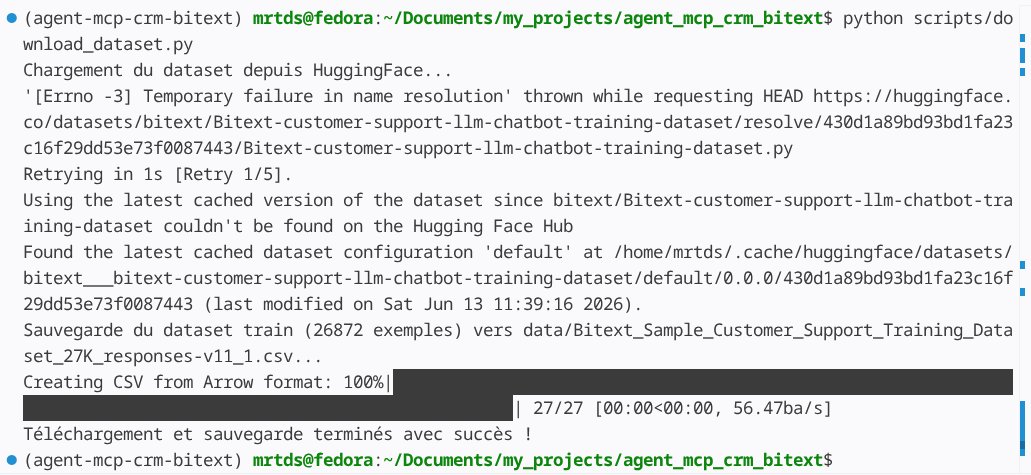
\includegraphics[width=\linewidth]{screenshoot/telechargement.png}

\subsection{Étape 2 : préparation des données}

La préparation des données est réalisée avec :

\begin{lstlisting}
scripts/prepare_data.py
\end{lstlisting}

Cette étape effectue plusieurs traitements :

\begin{itemize}
    \item chargement du CSV Bitext ;
    \item remplacement des templates comme \texttt{\{\{Order Number\}\}} ou \texttt{\{\{Website URL\}\}} ;
    \item création de colonnes nettoyées ;
    \item split stratifié train/validation/test ;
    \item export des fichiers CSV ;
    \item génération des fichiers JSONL.
\end{itemize}

Les fichiers générés sont :

\begin{lstlisting}
data/bitext_train.csv
data/bitext_val.csv
data/bitext_test.csv
data/bitext_train_formatted.jsonl
data/bitext_val_formatted.jsonl
\end{lstlisting}

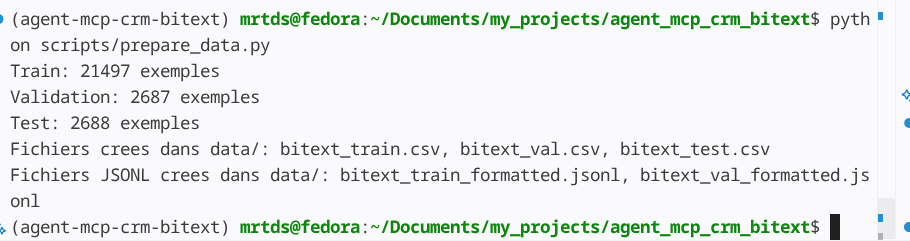
\includegraphics[width=\linewidth]{screenshoot/preparation.png}

\subsection{Étape 3 : analyse exploratoire}

L'analyse exploratoire a permis d'étudier la distribution des intentions, les catégories, les flags comportementaux, les longueurs de textes et les templates présents dans les messages.

% \screenshotplaceholder{Capture 3 -- Distribution des catégories et des intentions}{Graphique d'analyse exploratoire du dataset.}
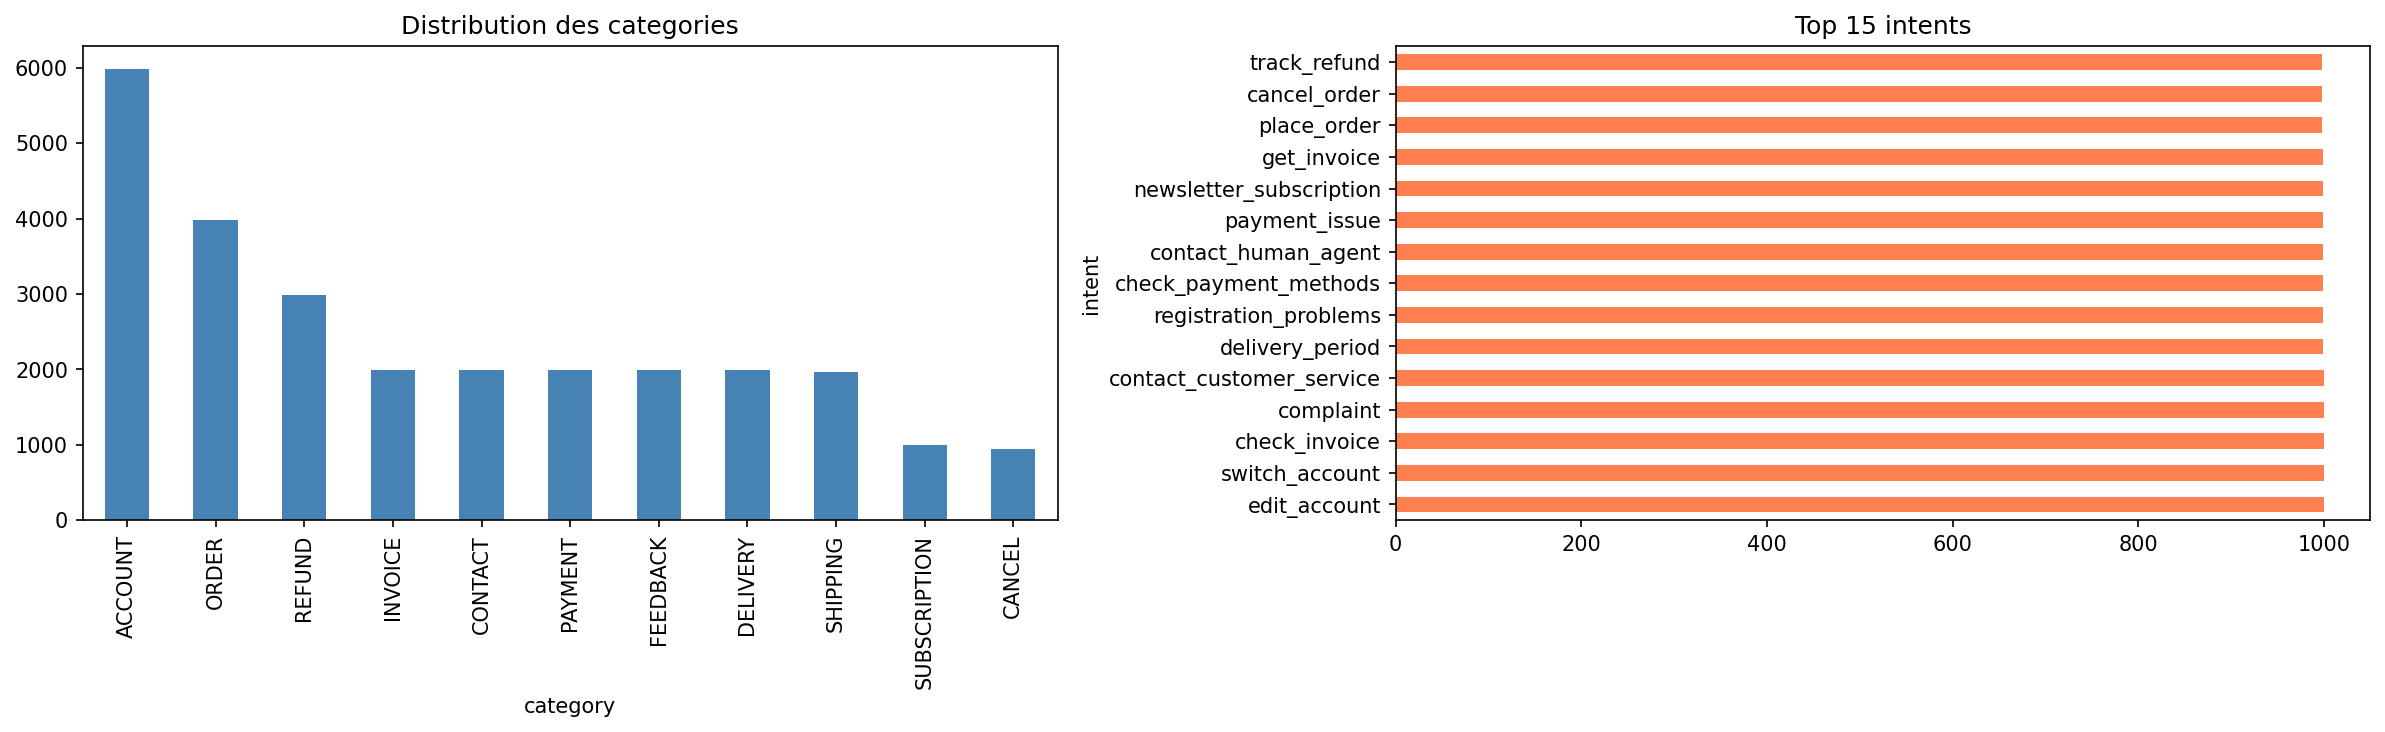
\includegraphics[width=\linewidth]{distribution_dataset.png}

% \screenshotplaceholder{Capture 4 -- Distribution des longueurs de texte}{Graphique des longueurs des instructions et réponses.}
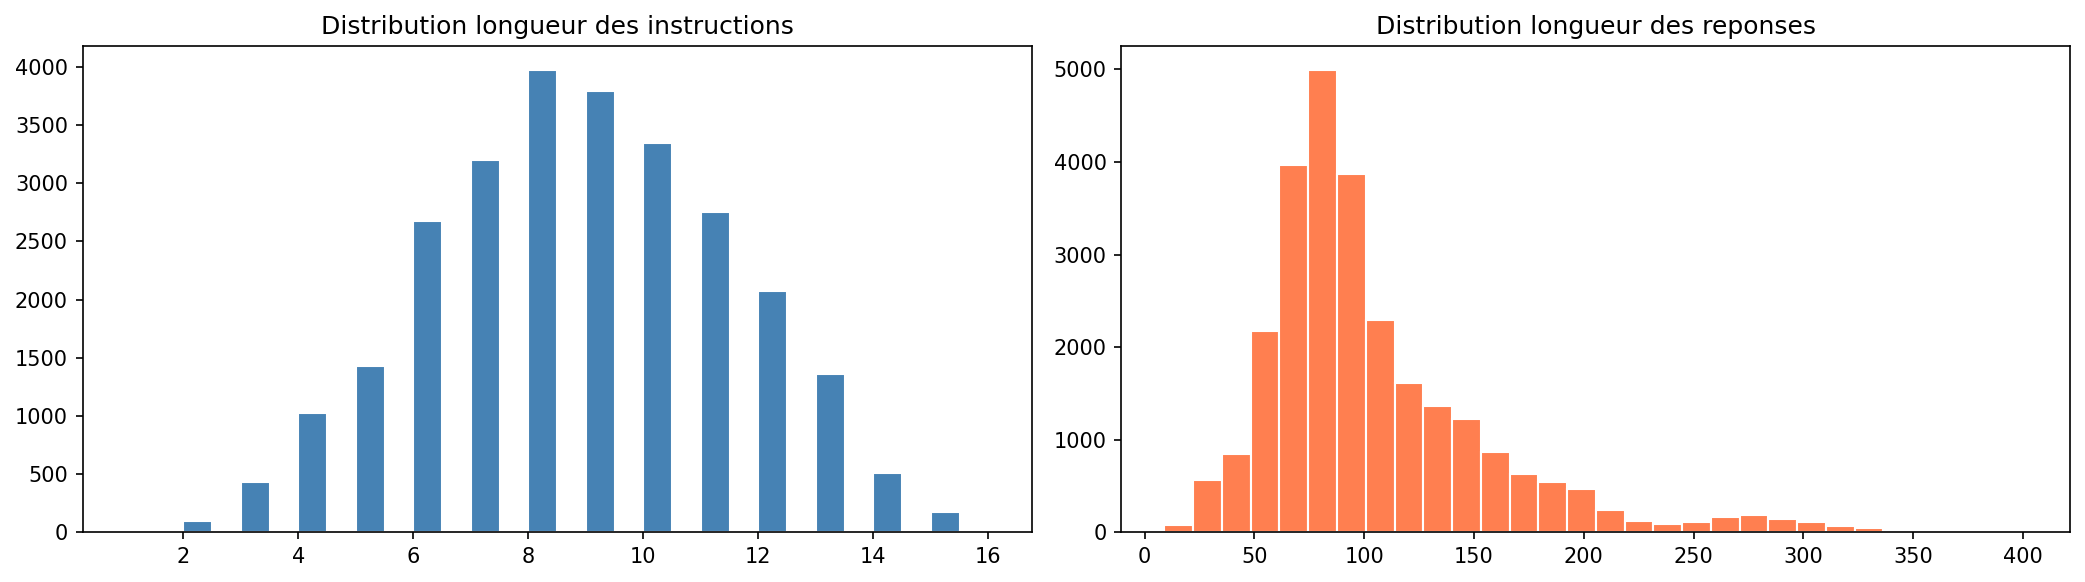
\includegraphics[width=\linewidth]{longueurs_texte.png}

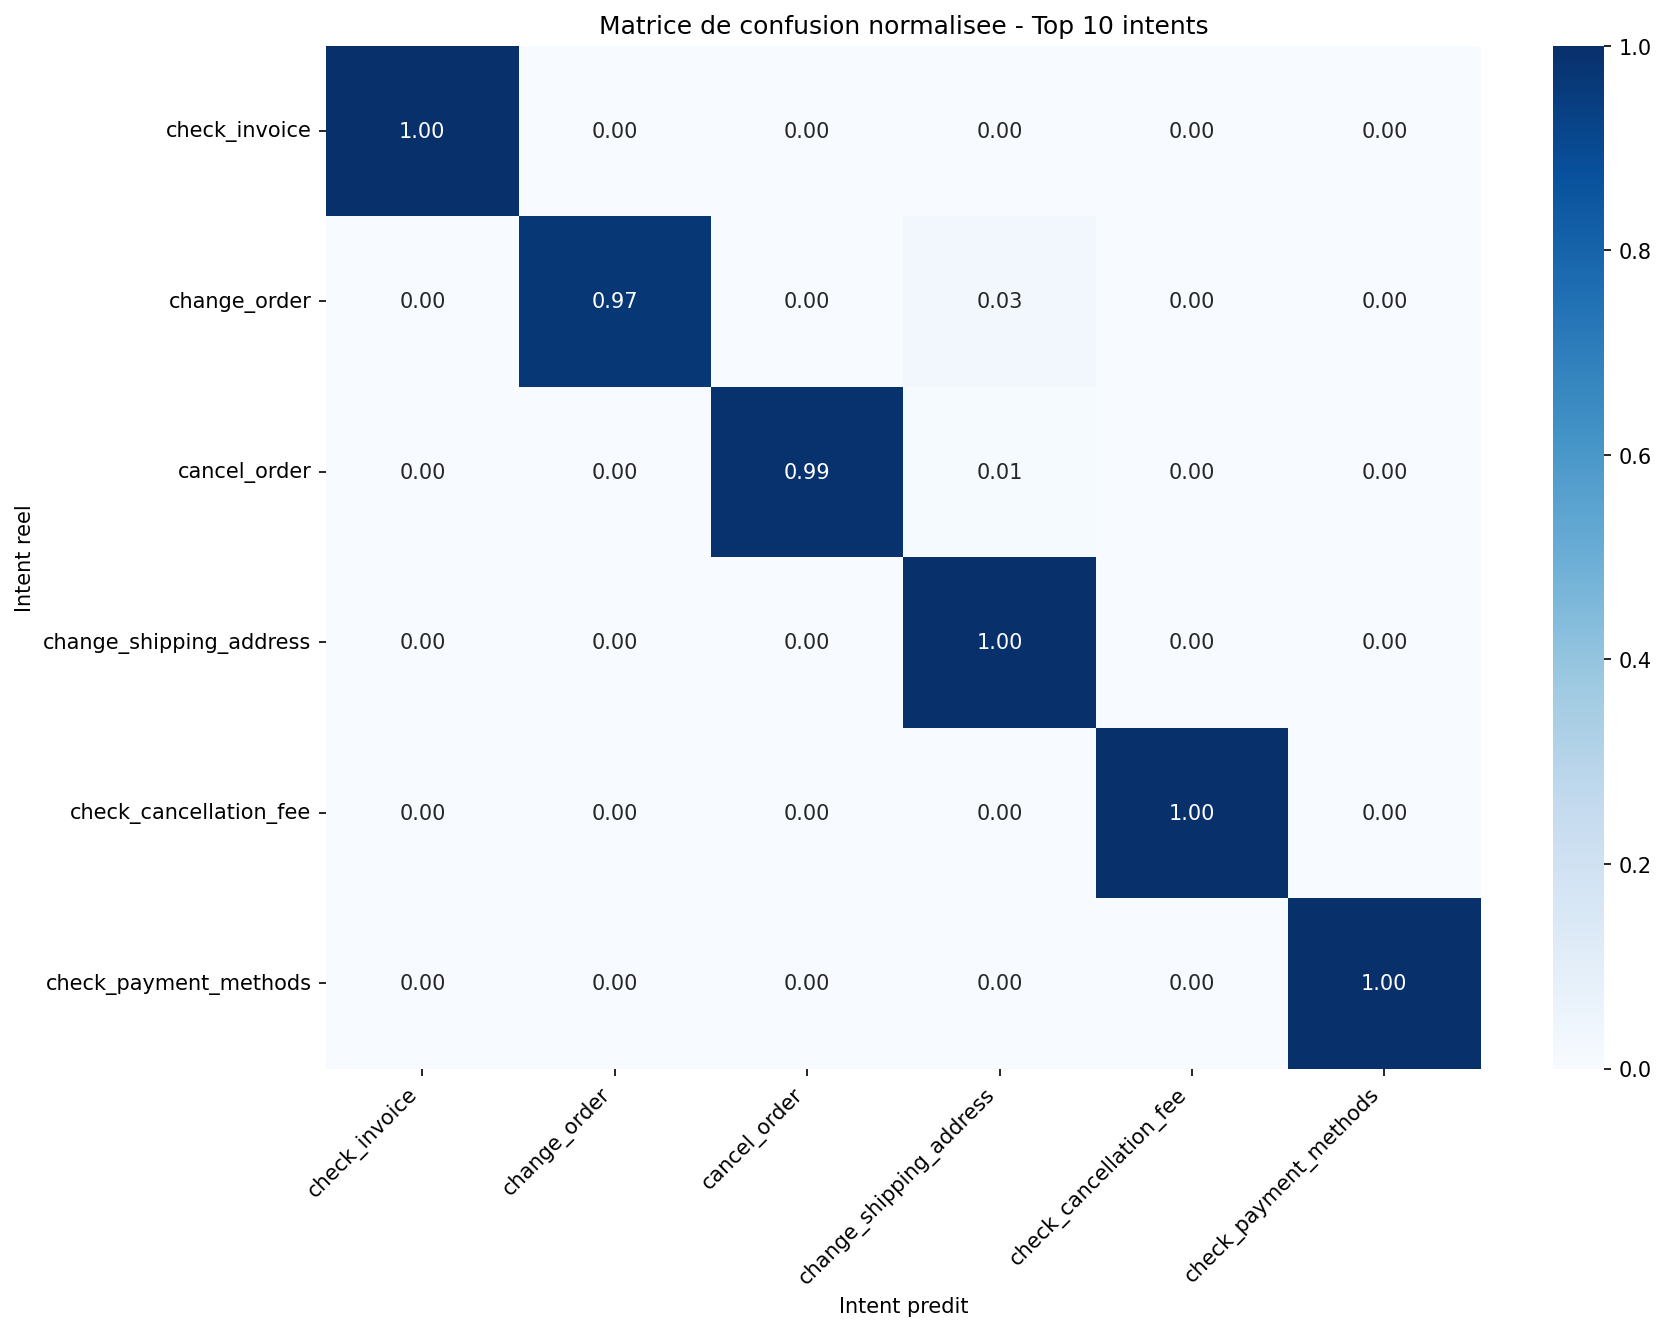
\includegraphics[width=\linewidth]{confusion_matrix.png}

\section{Architecture MCP}

Le projet repose sur un mapping explicite entre les intentions du dataset Bitext et des tools MCP. Ce mapping est défini dans :

\begin{lstlisting}
src/mcp_mapping.py
\end{lstlisting}

Exemples :

\begin{lstlisting}
cancel_order -> cancel_order(order_id)
track_order -> get_order_status(order_id)
change_shipping_address -> update_shipping_address(order_id, new_address)
get_refund -> process_refund(order_id, reason)
contact_human_agent -> escalate_to_human(reason)
\end{lstlisting}

Les tools sont implémentés dans :

\begin{lstlisting}
src/tools.py
\end{lstlisting}

Ils sont actuellement simulés, mais fonctionnels. Ils retournent des dictionnaires Python représentant des réponses CRM.

% \screenshotplaceholder{Capture 6 -- Mapping intent vers tool MCP}{Extrait du mapping ou exemple d'appel d'un tool.}
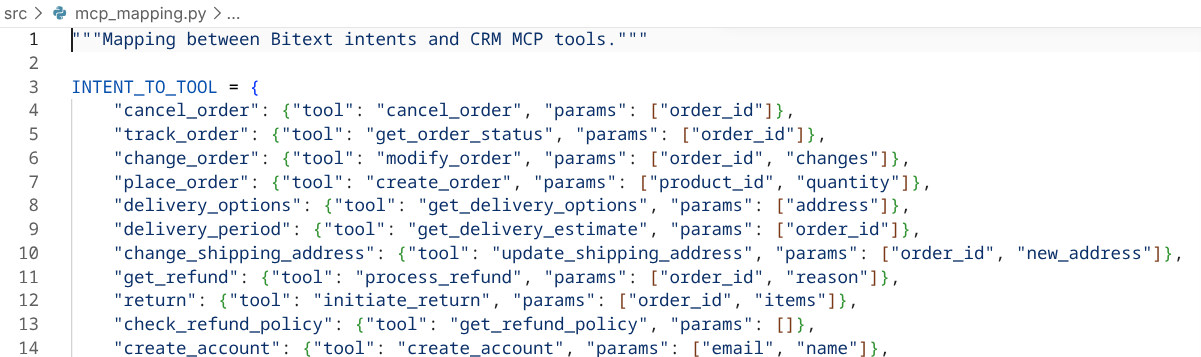
\includegraphics[width=\linewidth]{screenshoot/mapping.png}

\chapter{Modèles de classification et génération}

\section{Classificateur principal : TF-IDF + LogisticRegression}

Le classificateur principal du projet repose sur :

\begin{lstlisting}
TF-IDF + LogisticRegression
\end{lstlisting}

Il est implémenté dans :

\begin{lstlisting}
src/classifier.py
\end{lstlisting}

Le pipeline utilise des unigrammes et bigrammes, un maximum de 10 000 features, une régression logistique et un entraînement supervisé sur la colonne \texttt{intent}.

Commande d'entraînement :

\begin{lstlisting}
python scripts/train_classifier.py
\end{lstlisting}

Le modèle entraîné est sauvegardé dans :

\begin{lstlisting}
data/intent_classifier.pkl
\end{lstlisting}

Ce choix est particulièrement adapté aux contraintes matérielles du projet, car il fonctionne efficacement sur CPU.

\section{Justification du choix}

Au départ, le projet envisageait un fine-tuning de modèle LLM, notamment avec QLoRA sur \texttt{Qwen/Qwen2.5-3B-Instruct}. Cependant, cette approche demande un GPU, comme une carte T4 sur Google Colab.

Or, l'environnement local disponible est principalement CPU. Le choix final a donc été d'utiliser \textbf{TF-IDF + LogisticRegression} pour la classification d'intentions, et de réserver Ollama à la reformulation de réponse.

\section{Variante Transformer}

Le projet intègre également une variante Transformer optionnelle. Les fichiers concernés sont :

\begin{lstlisting}
src/transformer_classifier.py
scripts/train_transformer_classifier.py
\end{lstlisting}

Le modèle par défaut est :

\begin{lstlisting}
google/bert_uncased_L-2_H-128_A-2
\end{lstlisting}

Il s'agit d'un mini-BERT léger, plus adapté au CPU qu'un grand modèle Transformer.

Le script permet également d'utiliser DistilBERT :

\begin{lstlisting}
python scripts/train_transformer_classifier.py --model-name distilbert-base-uncased
\end{lstlisting}

Cette variante est intéressante pour expérimenter avec des modèles deep learning, mais elle reste plus lourde que TF-IDF.

\section{Choix du modèle Ollama}

Le modèle Ollama recommandé dans la version finale est :

\begin{lstlisting}
qwen2.5:1.5b
\end{lstlisting}

Ce choix a été fait car il représente un bon compromis entre qualité de génération et performance sur CPU.

La configuration se trouve dans :

\begin{lstlisting}
src/config.py
\end{lstlisting}

avec :

\begin{lstlisting}
DEFAULT_OLLAMA_MODEL = "qwen2.5:1.5b"
FALLBACK_OLLAMA_MODEL = "qwen2.5:1.5b"
\end{lstlisting}

Le rôle d'Ollama dans la solution finale n'est pas de classifier l'intention. La classification est assurée par TF-IDF ou Transformer. Ollama sert uniquement à produire ou reformuler une réponse plus naturelle.

% \screenshotplaceholder{Capture 7 -- Vérification Ollama}{Vérification du modèle \texttt{qwen2.5:1.5b} installé localement.}
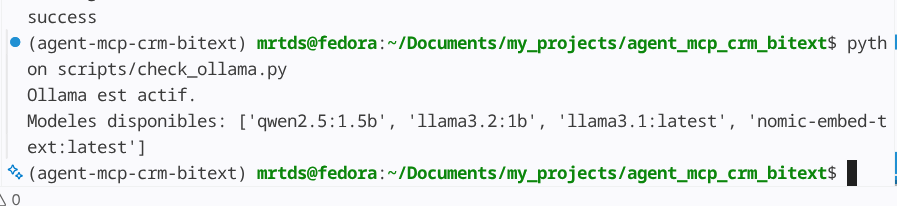
\includegraphics[width=\linewidth]{screenshoot/verification.png}

\chapter{Agent, API et interface utilisateur}

La classe principale de l'agent est :

\begin{lstlisting}
src/agent.py
\end{lstlisting}

Elle est représentée par :

\begin{lstlisting}
CRMAgent
\end{lstlisting}

Son rôle est d'orchestrer tout le pipeline :

\begin{enumerate}
    \item recevoir le message utilisateur ;
    \item classifier l'intention ;
    \item vérifier le score de confiance ;
    \item appliquer un fallback vers un agent humain si la confiance est faible ;
    \item exécuter le tool MCP correspondant ;
    \item générer ou retourner une réponse ;
    \item stocker l'historique de conversation.
\end{enumerate}

% \screenshotplaceholder{Capture 8 -- Test de l'agent}{Test de l'agent en ligne de commande avec \texttt{scripts/demo\_agent.py}.}
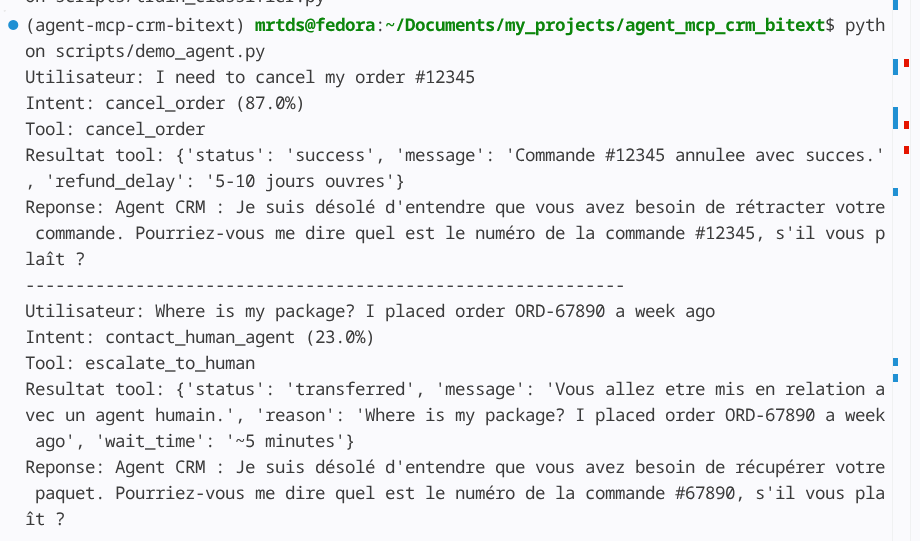
\includegraphics[width=\linewidth]{screenshoot/test_agent.png}

\section{API FastAPI}

L'API est implémentée dans :

\begin{lstlisting}
api.py
\end{lstlisting}

Elle expose plusieurs endpoints :

\begin{lstlisting}
GET /health
POST /chat
DELETE /session/{session_id}
GET /intents
\end{lstlisting}

\subsection{Endpoint /health}

Cet endpoint permet de vérifier que l'API est active.

\subsection{Endpoint /chat}

Cet endpoint permet d'envoyer un message à l'agent CRM.

\begin{lstlisting}
curl -X POST http://localhost:8000/chat ^
  -H "Content-Type: application/json" ^
  -d "{\"message\":\"I want to cancel my order number 12345\",\"session_id\":\"demo\"}"
\end{lstlisting}

\subsection{Endpoint /intents}

Cet endpoint permet de consulter la liste des intentions connues par le classificateur.

\subsection{Gestion des sessions}

L'API maintient des sessions en mémoire avec un dictionnaire Python. Cela permet de garder un historique conversationnel par session.

% \screenshotplaceholder{Capture 9 -- Lancement de l'API}{Terminal avec \texttt{uvicorn api:app --reload --port 8000}.}
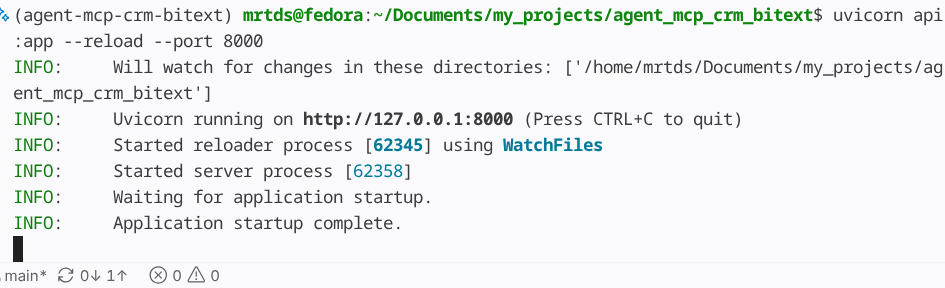
\includegraphics[width=\linewidth]{screenshoot/api.png}
% \screenshotplaceholder{Capture 10 -- Swagger FastAPI}{Interface \texttt{/docs}.}
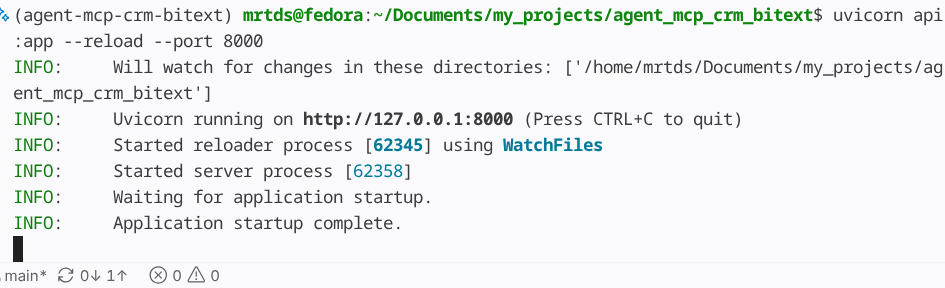
\includegraphics[width=\linewidth]{screenshoot/api.png}
% \screenshotplaceholder{Capture 11 -- Test du endpoint /chat}{Requête de test d'un message client.}
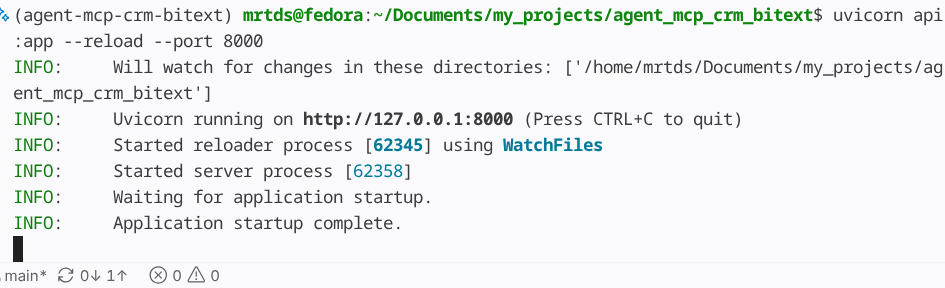
\includegraphics[width=\linewidth]{screenshoot/api.png}
% \screenshotplaceholder{Capture 12 -- Liste des intents}{Résultat du endpoint \texttt{/intents}.}
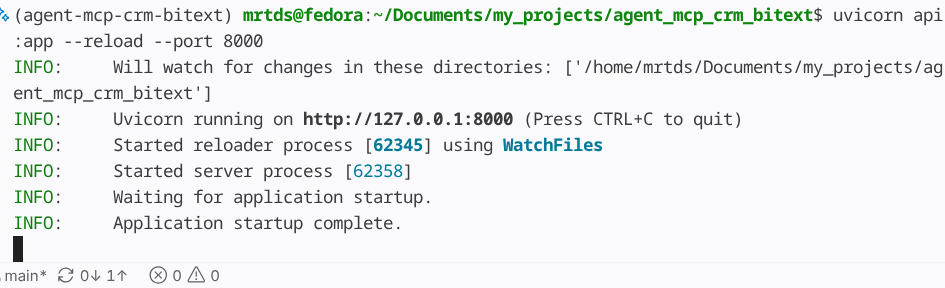
\includegraphics[width=\linewidth]{screenshoot/api.png}

\section{Interface Streamlit}

Une contribution importante de finalisation a été l'ajout d'une interface utilisateur interactive avec Streamlit. Le fichier concerné est :

\begin{lstlisting}
streamlit_app.py
\end{lstlisting}

Cette interface permet de rendre le système plus accessible, plus démontrable et plus compréhensible. Elle est connectée à l'API FastAPI et permet de tester le pipeline complet sans passer par la ligne de commande.

\subsection{Fonctionnalités principales}

L'interface permet :

\begin{itemize}
    \item de configurer l'URL de l'API FastAPI ;
    \item de vérifier si l'API est connectée ;
    \item de consulter la liste des intents disponibles ;
    \item de saisir un message client personnalisé ;
    \item de sélectionner un exemple prédéfini ;
    \item d'envoyer le message à l'API ;
    \item d'afficher l'intention détectée ;
    \item d'afficher le score de confiance ;
    \item d'afficher le tool MCP appelé ;
    \item de consulter le résultat technique du tool ;
    \item de suivre l'historique des interactions ;
    \item d'exporter l'historique au format CSV.
\end{itemize}

\subsection{Seuil de confiance}

L'interface intègre un seuil de confiance configurable, fixé par défaut à 0.70. Si le score de confiance est inférieur à ce seuil, l'interface recommande une redirection vers un agent humain.

\subsection{Dashboard de session}

Un dashboard permet de suivre le nombre de messages analysés, la confiance moyenne, le nombre d'intentions détectées, le nombre de cas nécessitant une escalade, la répartition des intentions et l'historique technique.

\subsection{Exemple de test}

Un exemple de test concluant a été réalisé avec le message :

\begin{lstlisting}
I want to cancel my order number 12345
\end{lstlisting}

Le système a détecté l'intention \texttt{cancel\_order} et a appelé le tool \texttt{cancel\_order}.

% \screenshotplaceholder{Capture 13 -- Interface Streamlit}{Page d'accueil de l'interface.}
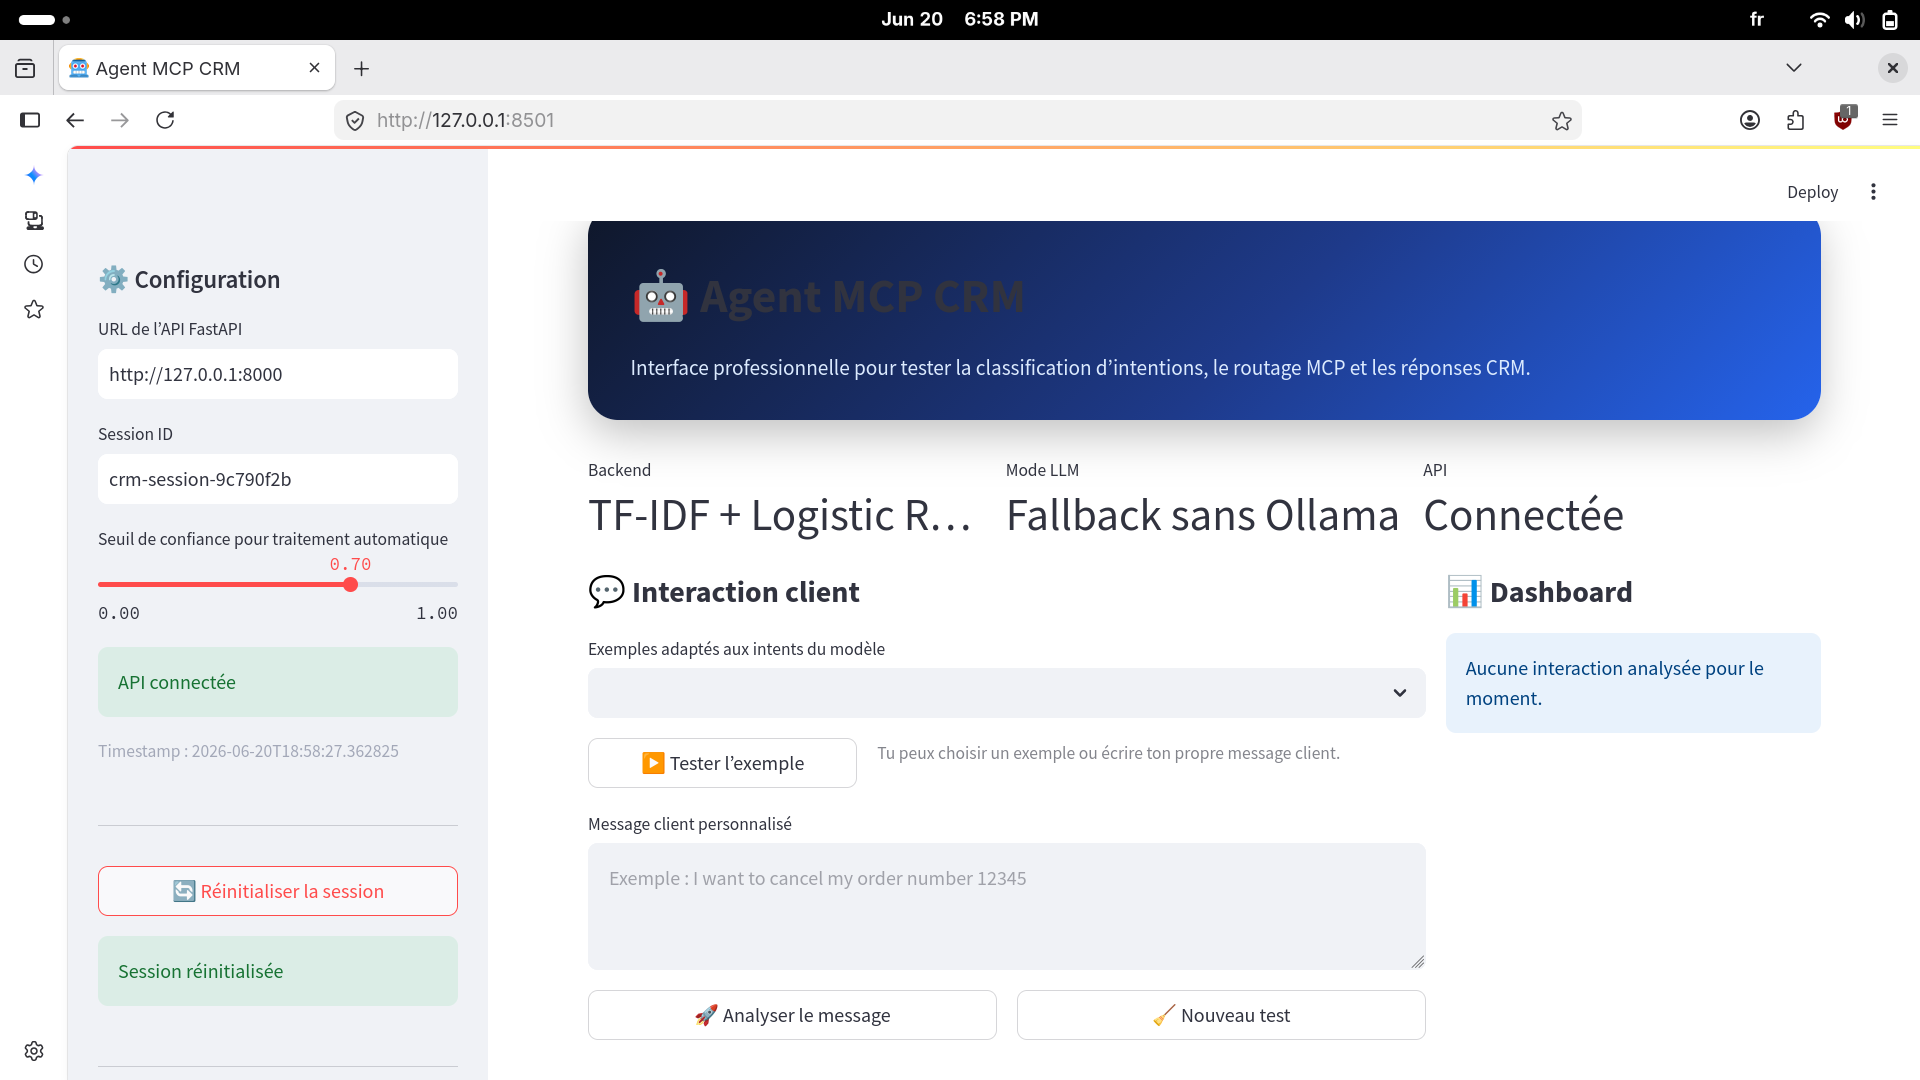
\includegraphics[width=\linewidth]{screenshoot/streamlit.png}
% \screenshotplaceholder{Capture 14 -- Configuration API}{Sidebar avec URL API, session ID et état de connexion.}
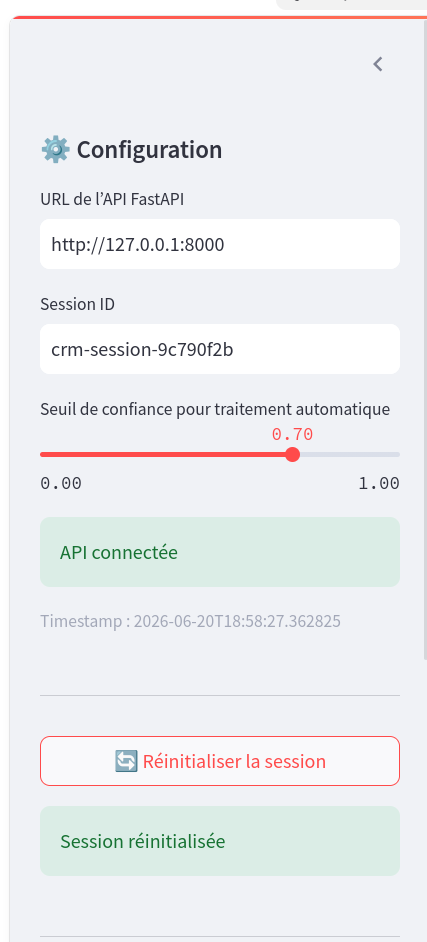
\includegraphics[height=17cm, width=\linewidth]{screenshoot/config_api.png}
% \screenshotplaceholder{Capture 15 -- Message client}{Saisie d'un message client.}
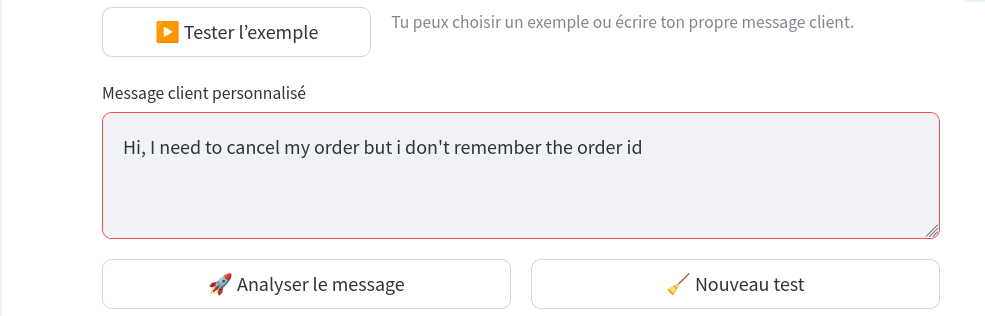
\includegraphics[width=\linewidth]{screenshoot/client_msg.png}
% \screenshotplaceholder{Capture 16 -- Résultat de classification}{Intent, score de confiance et niveau.}
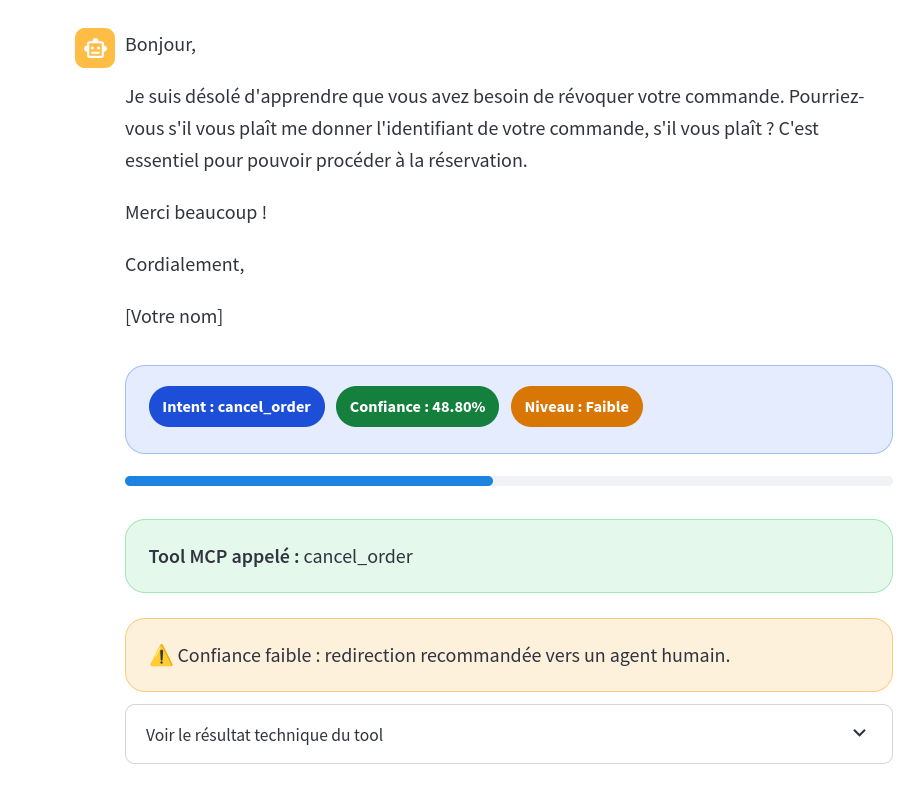
\includegraphics[width=\linewidth]{screenshoot/result_msg.png}
% \screenshotplaceholder{Capture 17 -- Tool MCP appelé}{Affichage du tool appelé et du résultat technique.}
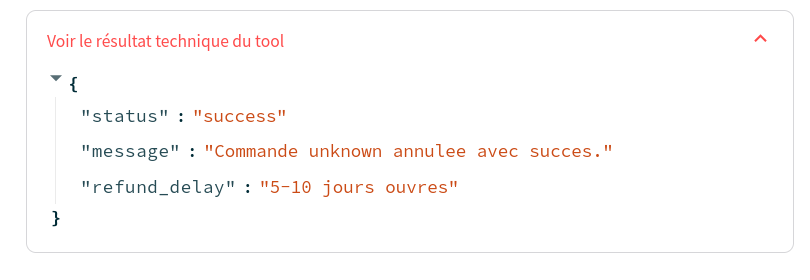
\includegraphics[width=\linewidth]{screenshoot/result_techn.png}
% \screenshotplaceholder{Capture 18 -- Dashboard Streamlit}{Statistiques de session.}
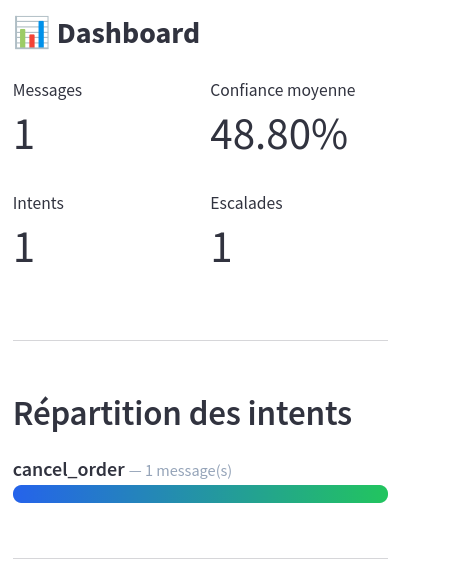
\includegraphics[width=\linewidth]{screenshoot/stat_session.png}
% \screenshotplaceholder{Capture 19 -- Export CSV}{Bouton de téléchargement de l'historique.}
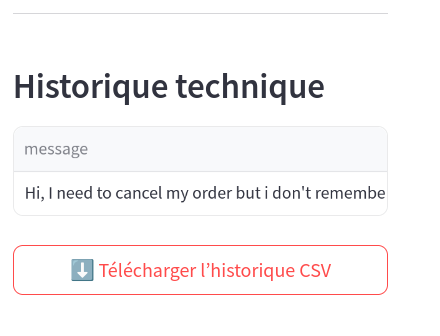
\includegraphics[width=\linewidth]{screenshoot/export_excel.png}

\chapter{Dépendances et déploiement}

Deux fichiers de dépendances sont disponibles.

\section{requirements.txt}

Ce fichier contient les dépendances complètes, notamment \texttt{pandas}, \texttt{matplotlib}, \texttt{seaborn}, \texttt{scikit-learn}, \texttt{fastapi}, \texttt{uvicorn}, \texttt{pydantic}, \texttt{langchain}, \texttt{langchain-ollama}, \texttt{datasets}, \texttt{transformers}, \texttt{torch} et \texttt{evaluate}.

\section{requirements\_light.txt}

Ce fichier contient une version plus légère pour l'API et l'interface Streamlit. Il est plus adapté aux machines à ressources limitées lorsqu'on ne souhaite pas entraîner de modèle Transformer.

\section{Déploiement}

\subsection{Lancement local}

Pour lancer l'API :

\begin{lstlisting}
uvicorn api:app --reload --port 8000
\end{lstlisting}

Pour lancer Streamlit :

\begin{lstlisting}
streamlit run streamlit_app.py
\end{lstlisting}

\subsection{Mode sans Ollama}

\begin{lstlisting}
$env:CRM_AGENT_USE_OLLAMA="false"
uvicorn api:app --reload --port 8000
\end{lstlisting}

\subsection{Mode avec Ollama}

\begin{lstlisting}
ollama serve
ollama pull qwen2.5:1.5b
uvicorn api:app --reload --port 8000
\end{lstlisting}

\subsection{Docker}

\begin{lstlisting}
docker build -t agent-crm .
docker run -p 8000:8000 -e CRM_AGENT_USE_OLLAMA=false agent-crm
\end{lstlisting}

% \screenshotplaceholder{Capture 20 -- Lancement FastAPI}{Terminal de lancement de FastAPI.}
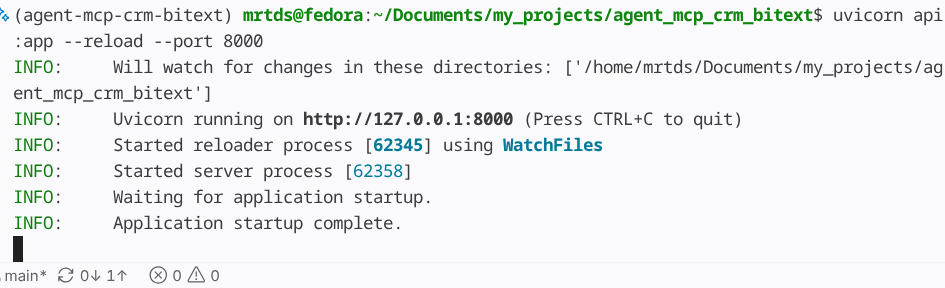
\includegraphics[width=\linewidth]{screenshoot/api.png}
% \screenshotplaceholder{Capture 21 -- Lancement Streamlit}{Terminal de lancement de Streamlit.}
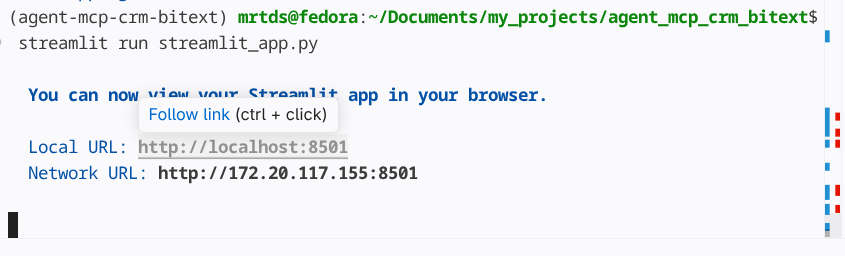
\includegraphics[width=\linewidth]{screenshoot/doc_streamlit.png}
% \screenshotplaceholder{Capture 22 -- Build Docker}{Commande \texttt{docker build}.}
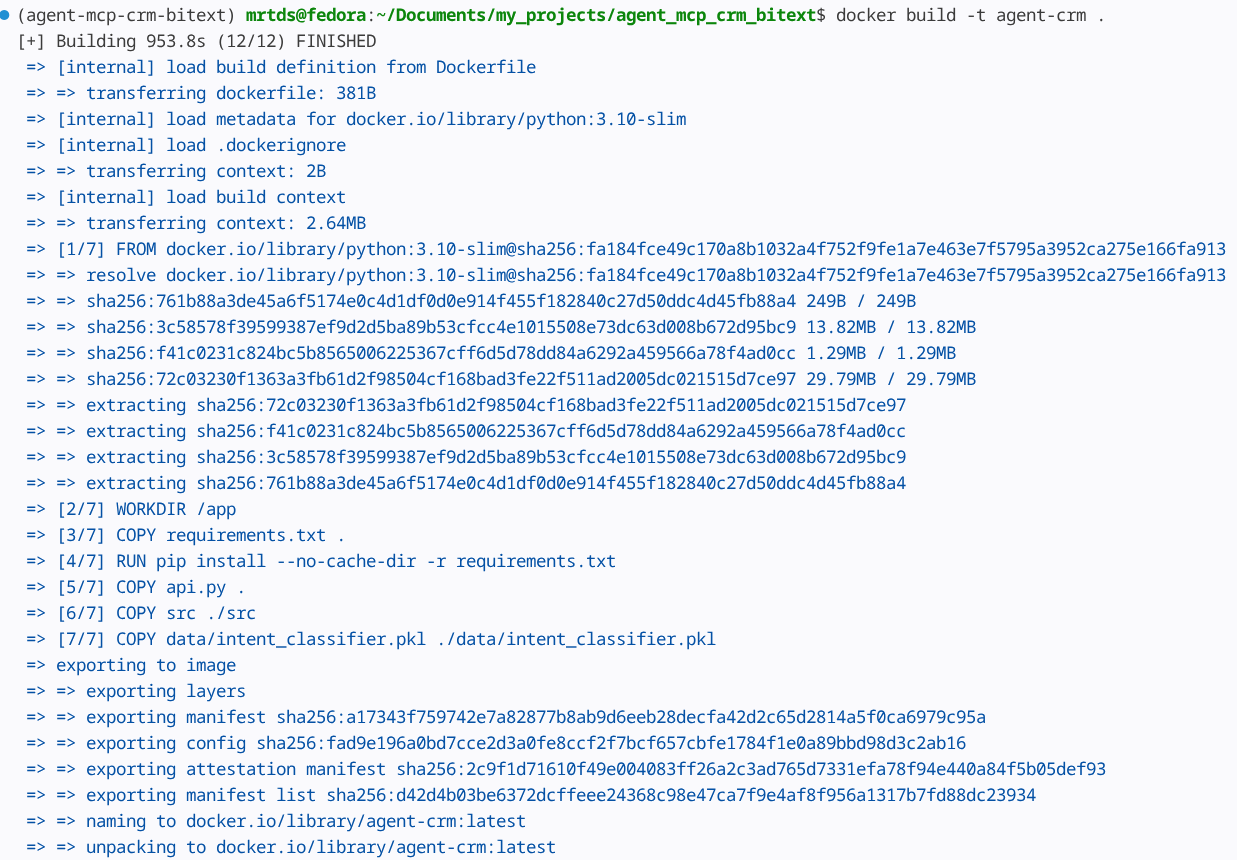
\includegraphics[width=\linewidth]{screenshoot/doc_build.png}
% \screenshotplaceholder{Capture 23 -- Conteneur Docker}{Commande \texttt{docker run}.}
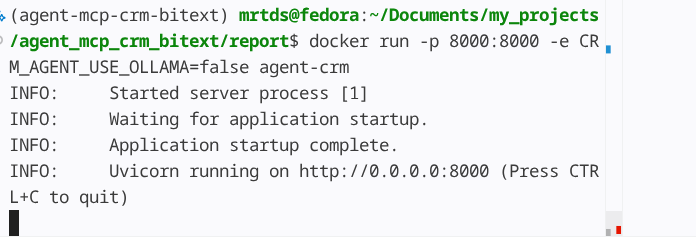
\includegraphics[width=\linewidth]{screenshoot/doc_run.png}

\chapter{Évaluation, bilan et perspectives}

\section{Évaluation du classificateur}

Le script :

\begin{lstlisting}
scripts/evaluate_classifier.py
\end{lstlisting}

permet de calculer l'accuracy globale, la confiance moyenne, le ratio d'exemples avec confiance supérieure à 80\%, un rapport de classification et une matrice de confusion.

\section{Tests fonctionnels}

Les tests fonctionnels portent sur la préparation des données, l'entraînement du classificateur, le chargement du modèle, l'appel des tools MCP, le fonctionnement de l'API, le fonctionnement de l'interface Streamlit, le routage correct des intents et la gestion des faibles scores de confiance.

\section{Tests de cas limites}

Les cas limites prévus incluent :

\begin{itemize}
    \item message vide ;
    \item message très court ;
    \item faute de frappe ;
    \item intention multiple ;
    \item demande hors périmètre ;
    \item message agressif ;
    \item absence de numéro de commande.
\end{itemize}

\section{État final d'avancement}

\subsection{Éléments finalisés}

\begin{itemize}
    \item Le notebook initial a été transformé en projet Python modulaire.
    \item Le dataset Bitext est intégré dans un workflow reproductible.
    \item Le script de téléchargement du dataset a été ajouté.
    \item Les données peuvent être préparées automatiquement.
    \item Le classificateur TF-IDF est entraînable localement.
    \item Le modèle est sauvegardé dans \texttt{data/intent\_classifier.pkl}.
    \item L'agent CRM est implémenté.
    \item Le mapping intent vers tool MCP est complet.
    \item Les tools MCP sont simulés et fonctionnels.
    \item L'API FastAPI est connectée au vrai agent.
    \item L'interface Streamlit est disponible.
    \item Ollama est configuré avec \texttt{qwen2.5:1.5b}.
    \item Le mode sans Ollama est disponible.
    \item Le mode Transformer optionnel est disponible.
    \item La documentation README a été structurée en étapes.
\end{itemize}

\subsection{Éléments partiellement réalisés}

\begin{itemize}
    \item Le fine-tuning complet d'un LLM avec QLoRA n'a pas été retenu pour l'exécution locale CPU.
    \item Le dataset Telco Churn n'a pas encore été intégré comme tool MCP.
    \item Les tools CRM restent des stubs, non connectés à un vrai système métier.
    \item Le modèle Transformer reste optionnel et expérimental.
    \item La persistance des sessions est en mémoire, sans Redis ou base de données.
\end{itemize}

\section{Limites actuelles}

Le projet reste perfectible sur plusieurs points :

\begin{itemize}
    \item la classification peut être moins robuste sur des messages réels très ambigus ;
    \item les intentions multiples ne sont pas encore gérées ;
    \item l'extraction des paramètres repose sur des règles simples ;
    \item les tools MCP ne sont pas connectés à un vrai CRM ;
    \item la mémoire conversationnelle est limitée ;
    \item l'interface Streamlit pourrait encore exposer plus d'options de configuration.
\end{itemize}

\section{Perspectives d'amélioration}

Plusieurs pistes sont possibles pour faire évoluer le projet :

\begin{itemize}
    \item intégrer le dataset Telco Churn ;
    \item ajouter un tool \texttt{predict\_churn(customer\_id)} ;
    \item améliorer l'extraction d'entités ;
    \item gérer les intentions multiples ;
    \item connecter les stubs MCP à un vrai backend CRM ;
    \item ajouter une persistance Redis ou SQLite ;
    \item améliorer l'interface Streamlit ;
    \item calibrer les seuils de confiance ;
    \item tester DistilBERT ou une architecture embeddings.
\end{itemize}

\section{Liste des captures d'écran à intégrer}

\begin{longtable}{|p{0.15\textwidth}|p{0.75\textwidth}|}
\hline
\textbf{Capture} & \textbf{Description} \\
\hline
1 & Téléchargement du dataset avec \texttt{download\_dataset.py}. \\
\hline
2 & Préparation des données avec \texttt{prepare\_data.py}. \\
\hline
3 & Fichiers générés dans le dossier \texttt{data/}. \\
\hline
4 & Distribution des catégories et intentions. \\
\hline
5 & Matrice de confusion. \\
\hline
6 & Entraînement du classificateur. \\
\hline
7 & Vérification Ollama. \\
\hline
8 & Démo agent en ligne de commande. \\
\hline
9 & Lancement FastAPI. \\
\hline
10 & Swagger FastAPI. \\
\hline
11 & Test du endpoint \texttt{/chat}. \\
\hline
12 & Interface Streamlit : accueil. \\
\hline
13 & Configuration API dans Streamlit. \\
\hline
14 & Test d'un message client. \\
\hline
15 & Résultat de classification. \\
\hline
16 & Tool MCP appelé. \\
\hline
17 & Dashboard Streamlit. \\
\hline
18 & Historique technique. \\
\hline
19 & Export CSV. \\
\hline
20 & Build Docker. \\
\hline
21 & Conteneur Docker lancé. \\
\hline
\end{longtable}

\chapter*{Conclusion générale}
\addcontentsline{toc}{chapter}{Conclusion générale}

Le projet \textbf{Agent MCP CRM Bitext} a évolué d'un notebook expérimental vers une application modulaire complète. La solution finale permet de traiter des messages clients, de détecter leur intention, d'appeler un tool CRM correspondant, puis de produire une réponse exploitable.

La solution repose sur une architecture pragmatique adaptée aux ressources disponibles :

\begin{lstlisting}
TF-IDF + LogisticRegression pour la classification
Tools MCP pour la logique metier
FastAPI pour l'exposition du service
Streamlit pour la demonstration interactive
Ollama qwen2.5:1.5b pour la reformulation optionnelle
\end{lstlisting}

Le projet atteint donc son objectif principal : démontrer un agent CRM intelligent, modulaire et fonctionnel, capable de combiner classification d'intentions, routage MCP et interaction utilisateur.

Les contributions finales ont permis de renforcer la reproductibilité, l'ergonomie et la démonstrabilité du projet, notamment grâce au script de téléchargement automatique du dataset, à l'intégration d'un backend Transformer optionnel, au choix d'un modèle Ollama plus léger, à l'interface Streamlit, à la structuration complète du projet et à la documentation par étapes.

Même si certains points restent perfectibles, notamment l'intégration d'un vrai CRM et la gestion des intentions multiples, la version actuelle constitue une base solide pour une solution agentique CRM locale et extensible.

\section*{Résumé final}
\addcontentsline{toc}{section}{Résumé final}

Le projet finalisé peut être résumé ainsi :

\begin{lstlisting}
Un agent CRM intelligent capable de :
- comprendre une demande client ;
- identifier son intention ;
- appeler un outil metier MCP ;
- retourner une reponse structuree ;
- etre teste via API ou interface Streamlit ;
- fonctionner sur CPU avec un modele leger.
\end{lstlisting}

La solution est adaptée aux contraintes matérielles du projet et reste évolutive pour de futures améliorations.

\end{document}
